%%% Template originaly created by Karol Kozioł (mail@karol-koziol.net) and modified for ShareLaTeX use

\documentclass[a4paper,fleqn,11pt]{article}

\usepackage[T1]{fontenc}
\usepackage[utf8]{inputenc}
\usepackage{graphicx}
\usepackage{xcolor}

\usepackage{tgtermes}

\usepackage[
pdftitle={EE698G - Probabilistic Mobile Robotics Assignment}, 
pdfauthor={Satya Prakash Panuganti, 14610},
colorlinks=true,linkcolor=blue,urlcolor=blue,citecolor=blue,bookmarks=true,
bookmarksopenlevel=2]{hyperref}
\usepackage{amsmath,amssymb,amsthm,textcomp}
\usepackage{enumerate}
\usepackage{multicol}
\usepackage{tikz}

\usepackage{geometry}
\geometry{total={210mm,297mm},
left=25mm,right=25mm,%
bindingoffset=0mm, top=20mm,bottom=20mm}

\usepackage{ mathrsfs }

\linespread{1.3}

\newcommand{\linia}{\rule{\linewidth}{0.5pt}}

% custom theorems if needed
\newtheoremstyle{mytheor}
    {1ex}{1ex}{\normalfont}{0pt}{\scshape}{.}{1ex}
    {{\thmname{#1 }}{\thmnumber{#2}}{\thmnote{ (#3)}}}

\theoremstyle{mytheor}
\newtheorem{defi}{Definition}

% my own titles
\makeatletter
\renewcommand{\maketitle}{
\begin{center}
\vspace{2ex}
{\huge \textsc{\@title}}
\vspace{1ex}
\\
\linia\\
\@author \hfill \@date
\vspace{4ex}
\end{center}
}
\makeatother
%%%

% custom footers and headers
\usepackage{fancyhdr,lastpage}
\pagestyle{fancy}
\lhead{}
\chead{}
\rhead{}
\lfoot{Assignment 2}
\cfoot{}
\rfoot{Page \thepage\ /\ \pageref*{LastPage}}
\renewcommand{\headrulewidth}{0pt}
\renewcommand{\footrulewidth}{0pt}
%

%%%----------%%%----------%%%----------%%%----------%%%

\begin{document}

\title{EE604A - Digital Image Processing Assignment}

\author{Satya Prakash Panuganti, 14610}

\date{31 August, 2017}

\maketitle

\section*{Image Sources}
Sunset  (high.jpg)  : \url{https://www.flickr.com/photos/mediaflex/4190084346} \\
Carving (low.jpg)   : \url{https://www.flickr.com/photos/30440933@N06/2847993403} \\
Dog     (small.jpg) : \url{https://res.cloudinary.com/rover-com/image/upload/a_exif,c_fill,f_jpg,fl_progressive,g_face:center,h_100,q_80,w_100/remote/images/pets/4NpPzO8N/50e4a023d9/original.jpg} \\
divyat.jpg 			 : Own work. Taken with permission.
\section*{Solution 1}
\subsection*{(a)}
Code has been written in two MATLAB\textregistered\ files :
\begin{itemize}
\item Q1\textbackslash lloyd\_max\_quantizer.m : The file contating the function.
\item Q1\textbackslash Q1.m : The script to perform the required tasks.
\end{itemize}
\subsection*{(b)}
The 4 representation levels are :

The corresponding transition levels are :

\subsection*{(c)}
\subsection*{(d)}
\subsection*{(e)}

\section*{Solution 2}

A C++ function, EE604A::histogram\_matching(), for histogram matching of cv::Mat images has been developed.
The code required for the matching function is present in :
\begin{itemize}
\item Q2\textbackslash src\textbackslash histogram\_matching.cxx
\item Q2\textbackslash src\textbackslash histogram\_matching.h 
\end{itemize}
A small program which uses the histogram matching function is present in Q2\textbackslash src\textbackslash Q2.cxx

In order to build and run the code, the following steps need to be followed :
\begin{enumerate}
\item Enter Q2\textbackslash src.
\item run build.sh (OpenCV needs to installed and a version of g++ supporting c++14 needs to be present)
\item Execute Q2 (the binary file) with the reference and target relative/absolute image paths. Eg. [./Q2 ../../images/high.jpg ../../images/low.jpg] or [./Q2 ../../images/low.jpg ../../images/high.jpg] (On Ubuntu)
\item The program can be closed by Ctrl+C on the terminal or by pressing 'q' when one of the image windows is open.
\end{enumerate}
REMARK : A simple plot of the the histograms can be obtained by toggling the third argument of the function EE604A::histogram\_matching() to true.

\subsection*{Results}
\begin{center}
Target : high.jpg, Reference : low.jpg \\
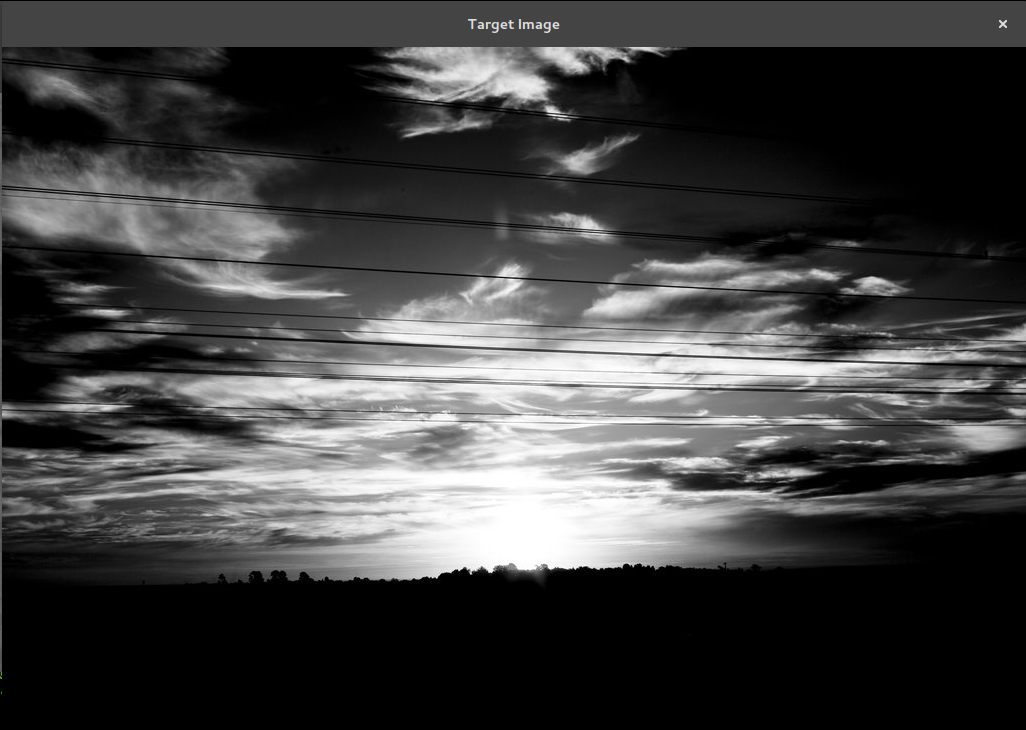
\includegraphics[scale= 0.25]{../results/target1.png}
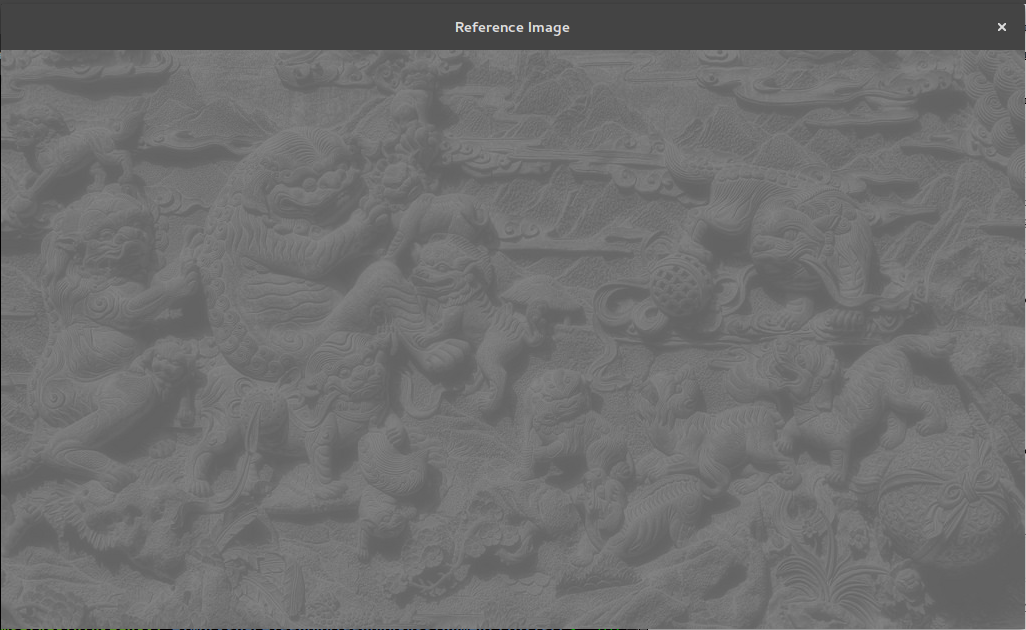
\includegraphics[scale= 0.25]{../results/reference1.png}
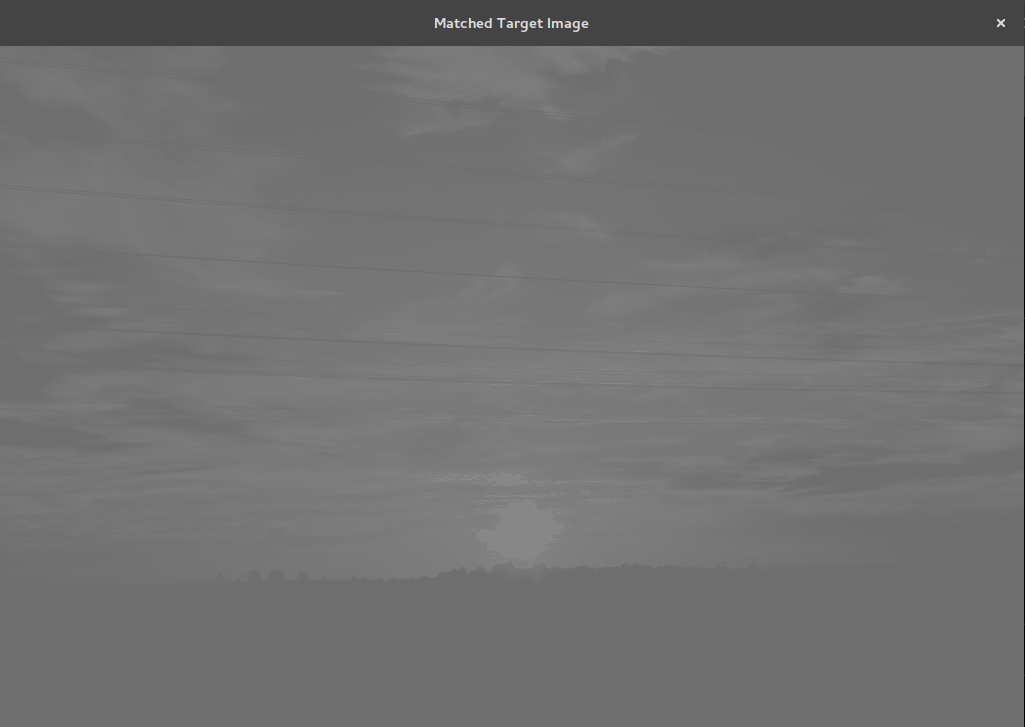
\includegraphics[scale= 0.25]{../results/matched1.png}
\end{center}
\begin{center}
Target : low.jpg, Reference : high.jpg \\
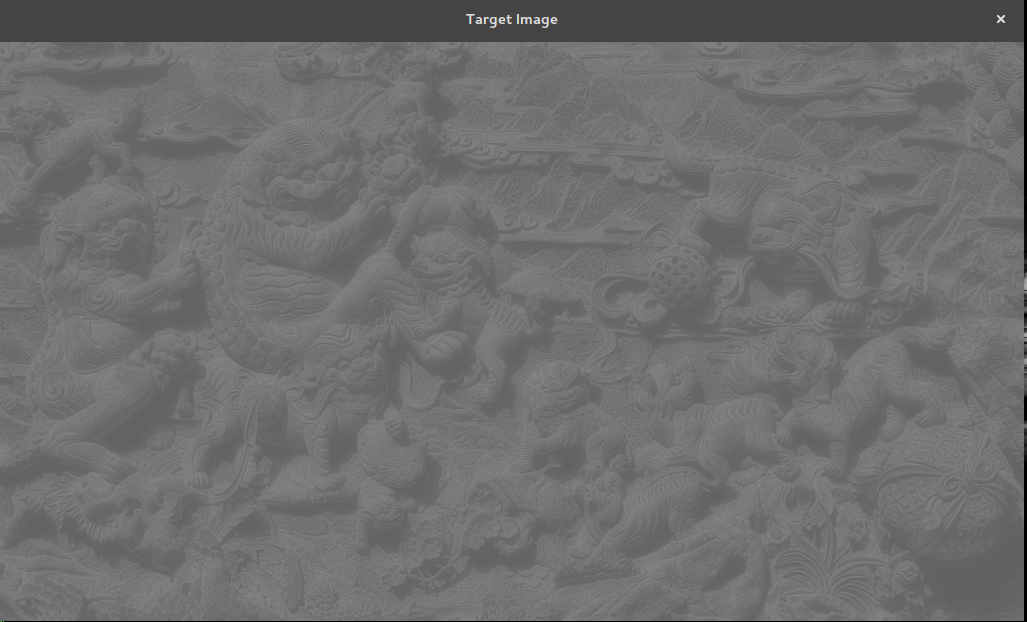
\includegraphics[scale= 0.25]{../results/target2.png}
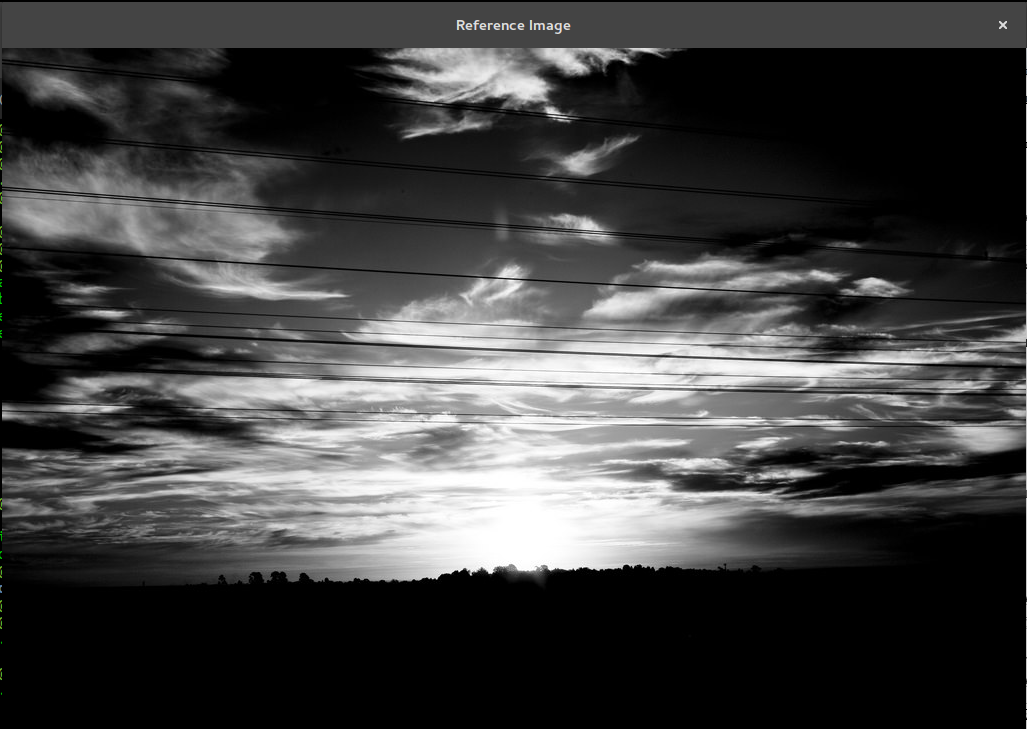
\includegraphics[scale= 0.25]{../results/reference2.png}
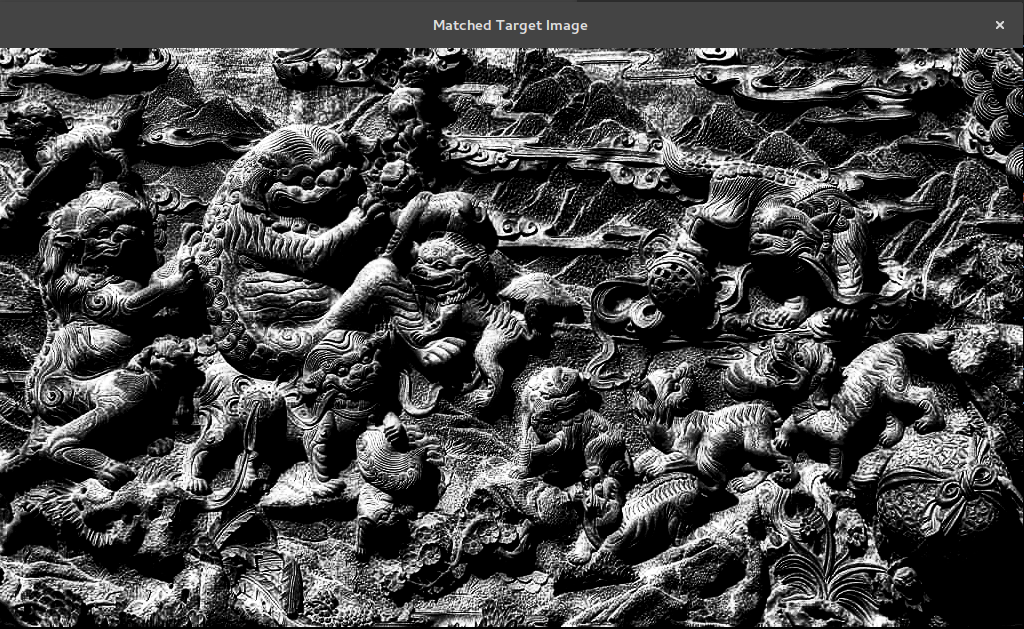
\includegraphics[scale= 0.25]{../results/matched2.png}
\end{center}

\section*{Solution 3}
Bilinear interpolation in a 8-connect neighborhood.
\section*{Solution 4}
$$\text{We are assuming that }\eta_i (x_1, y_1)\ and\ \eta_j (x_2, y_2)\text{ are independent if i }\neq j\ or\ x_1 \neq x_2\ or\ y_1 \neq y_w.$$
\begin{align}
\therefore\ if\ i \neq j,\ E[\eta_i(x, y)\eta_j(x, y)] & = 0
\end{align}
\begin{align*}
We\ have,\ g_i(x, y) & = f_i(x, y) + \eta_i(x, y) \\
Also,\ f_i(x, y) & = f(x, y) \\
Now,\ \hat{g}(x, y)& = \frac{1}{K} \Sigma_{i = 1}^K g_i(x, y) \\
& = \frac{1}{K}K f(x, y) + \frac{1}{K}\Sigma_{i = 1}^K \eta_i(x, y) \\
& = f(x, y) + \frac{1}{K}\Sigma_{i = 1}^K \eta_i(x, y) \\
Now,\ noise\ variance,\ E[(\hat{g(x, y)} - f(x, y))^2] & = E[(\frac{1}{K}\Sigma_{i = 1}^K \eta_i(x, y))^2] \\
& = \frac{1}{K^2}\Sigma_{i = 1}^K\Sigma_{j = 1}^K E[\eta_i(x, y)\eta_j(x, y)] \\
& = \frac{1}{K^2}\Sigma_{i = 1}^K E[\eta_i(x, y)^2] & from\ (1) \\
& = \frac{1}{K^2}\Sigma_{i = 1}^K \sigma^2 & \because\ E[\eta_i(x, y)^2] = \sigma^2 \\
& = \frac{\sigma^2}{K} \\
q.e.d
\end{align*}

\section*{Solution 5}

Let $f(x, y, z) : \Re^3 \rightarrow \Re$. Let $[u\ v\ w]^T$ be the position of $[x\ y\ z]^T$ in a rotated cooridnate frame.
The relationship between $[u\ v\ w]^T$ and $[x\ y\ z]^T$ is given by :
\begin{align}
\begin{bmatrix}
	u \\
	v \\
	w
\end{bmatrix} & =
	R
\begin{bmatrix}
	x \\
	y \\
	z
\end{bmatrix} \\
where,\ R & = [R_1\ R_2\ R_3] \\
& = \begin{bmatrix}
		R_{11} & R_{12} & R_{13} \\
		R_{21} & R_{22} & R_{23} \\
		R_{31} & R_{32} & R_{33}
	\end{bmatrix} \\
Known\ properties\ of\ R,\ |R_1| & = 1 \\
|R_2| & = 1 \\
R_1^T R_2 & = 0 \\
R_3  & = R_1 \times R_2 \\
\implies\ |R_3| & = 1 \\
R_1^T R_3 & = R_2^T R_3 = 0 \\
R^{-1} & = R^T \\
We\ can\ also\ write,\
\begin{bmatrix}
	x \\
	y \\
	z
\end{bmatrix} & =
	R^T
\begin{bmatrix}
	u \\
	v \\
	w
\end{bmatrix} & from\ (2),\ (9) \\
Now,\ \nabla^2 f(u, v, w) & = \frac{\partial^2 f}{\partial^2 u} +
							  \frac{\partial^2 f}{\partial^2 v} +
						      \frac{\partial^2 f}{\partial^2 w} \\
\frac{\partial f}{\partial u} & =
\frac{\partial f}{\partial x}\frac{\partial x}{\partial u} +
\frac{\partial f}{\partial y}\frac{\partial y}{\partial u} +
\frac{\partial f}{\partial z}\frac{\partial z}{\partial u} \\
& = R_{11}\frac{\partial f}{\partial x} +
	R_{12}\frac{\partial f}{\partial y} +
	R_{13}\frac{\partial f}{\partial z} & from\ (4), (10) \\
Similarily,\ \frac{\partial f}{\partial v}
& = R_{21}\frac{\partial f}{\partial x} +
	R_{22}\frac{\partial f}{\partial y} +
	R_{23}\frac{\partial f}{\partial z}\\
\ \frac{\partial f}{\partial w}
& = R_{31}\frac{\partial f}{\partial x} +
	R_{32}\frac{\partial f}{\partial y} +
	R_{33}\frac{\partial f}{\partial z}
\end{align}
\begin{align}
\therefore\ \frac{\partial^2 f}{\partial^2 u} & =
R_{11}
(\frac{\partial^2 f}{\partial^2 x} \frac{\partial x}{\partial u} +
 \frac{\partial^2 f}{\partial y \partial x} \frac{\partial y}{\partial u} +
 \frac{\partial^2 f}{\partial z \partial x} \frac{\partial z}{\partial u})\notag \\
& + R_{12}(\frac{\partial^2 f}{\partial x \partial y} \frac{\partial x}{\partial u}
  + \frac{\partial^2 f}{\partial^2 y} \frac{\partial y}{\partial u}
  +	 \frac{\partial^2 f}{\partial z \partial x} \frac{\partial z}{\partial u}) \notag \\
& + R_{13}(\frac{\partial^2 f}{\partial x \partial z} \frac{\partial x}{\partial u}
  + \frac{\partial^2 f}{\partial y \partial z} \frac{\partial y}{\partial u} 
  +	 \frac{\partial^2 f}{\partial^2 z} \frac{\partial z}{\partial u}) & from\ (13)\ and\ chain\ rule \\
& = R_{11}^2\frac{\partial^2 f}{\partial^2 x} +
	R_{11}R_{12}\frac{\partial^2 f}{\partial y \partial x} +
	R_{11}R_{13}\frac{\partial^2 f}{\partial z \partial x}\notag \\
& + R_{12}R_{11}\frac{\partial^2 f}{\partial x \partial y} +
	R_{12}^2\frac{\partial^2 f}{\partial^2 y} +
	R_{12}R_{13}\frac{\partial^2 f}{\partial z \partial y}\notag \\
& + R_{13}R_{11}\frac{\partial^2 f}{\partial x \partial z} +
	R_{13}R_{12}\frac{\partial^2 f}{\partial y \partial z} +
	R_{13}^2\frac{\partial^2 f}{\partial^2 z} & from\ (4), (10) \\
Similarily,\ \frac{\partial^2 f}{\partial^2 v} & =
	R_{21}^2\frac{\partial^2 f}{\partial^2 x} +
	R_{21}R_{22}\frac{\partial^2 f}{\partial y \partial x} +
	R_{21}R_{23}\frac{\partial^2 f}{\partial z \partial x}\notag \\
& + R_{22}R_{21}\frac{\partial^2 f}{\partial x \partial y} +
	R_{22}^2\frac{\partial^2 f}{\partial^2 y} +
	R_{22}R_{23}\frac{\partial^2 f}{\partial z \partial y}\notag \\
& + R_{23}R_{21}\frac{\partial^2 f}{\partial x \partial z} +
	R_{23}R_{22}\frac{\partial^2 f}{\partial y \partial z} +
	R_{23}^2\frac{\partial^2 f}{\partial^2 z} \\
\frac{\partial^2 f}{\partial^2 w} & =
	R_{31}^2\frac{\partial^2 f}{\partial^2 x} +
	R_{31}R_{32}\frac{\partial^2 f}{\partial y \partial x} +
	R_{31}R_{33}\frac{\partial^2 f}{\partial z \partial x}\notag \\
& + R_{32}R_{31}\frac{\partial^2 f}{\partial x \partial y} +
	R_{32}^2\frac{\partial^2 f}{\partial^2 y} +
	R_{32}R_{33}\frac{\partial^2 f}{\partial z \partial y}\notag \\
& + R_{33}R_{31}\frac{\partial^2 f}{\partial x \partial z} +
	R_{33}R_{32}\frac{\partial^2 f}{\partial y \partial z} +
	R_{33}^2\frac{\partial^2 f}{\partial^2 z}
\end{align}
On performing $(17) + (18) + (19)$, we get using (5), (6), (7), (9) and (10)
\begin{align}
\frac{\partial^2 f}{\partial^2 u} +
\frac{\partial^2 f}{\partial^2 v} +
\frac{\partial^2 f}{\partial^2 w} & =
\frac{\partial^2 f}{\partial^2 u} +
\frac{\partial^2 f}{\partial^2 v} +
\frac{\partial^2 f}{\partial^2 w}\\
\implies\ \nabla^2 f(u, v, w) & = \frac{\partial^2 f}{\partial^2 u} +
							  \frac{\partial^2 f}{\partial^2 v} +
						      \frac{\partial^2 f}{\partial^2 w} \\
						      & = \frac{\partial^2 f}{\partial^2 x} +
							  \frac{\partial^2 f}{\partial^2 y} +
						      \frac{\partial^2 f}{\partial^2 z} & from\ (22) \\
						      & =  \nabla^2 f(x, y, z)
\end{align}
\begin{align*}
q.e.d
\end{align*}
\section*{Solution 6}

A C++ file containds the code required to perform the required task.

In order to build and run the code, the following steps need to be followed :
\begin{enumerate}
\item Enter Q6\textbackslash src.
\item run build.sh (OpenCV needs to installed and a version of g++ supporting c++14 needs to be present)
\item Execute Q6 (the binary file) with the relative/absolute image path. Eg. [./Q6 ../../images/high.jpg] or [./Q2 ../../images/low.jpg ../../images/high.jpg] (On Ubuntu)
\item The program can be closed by Ctrl+C on the terminal or by pressing `q' when one of the image windows is open.
\end{enumerate}
REMARK : A simple plot of the the histograms can be obtained by toggling the third argument of the function EE604A::histogram\_matching() to true.
\subsection*{Results}
\begin{center}
divyat.jpg \\
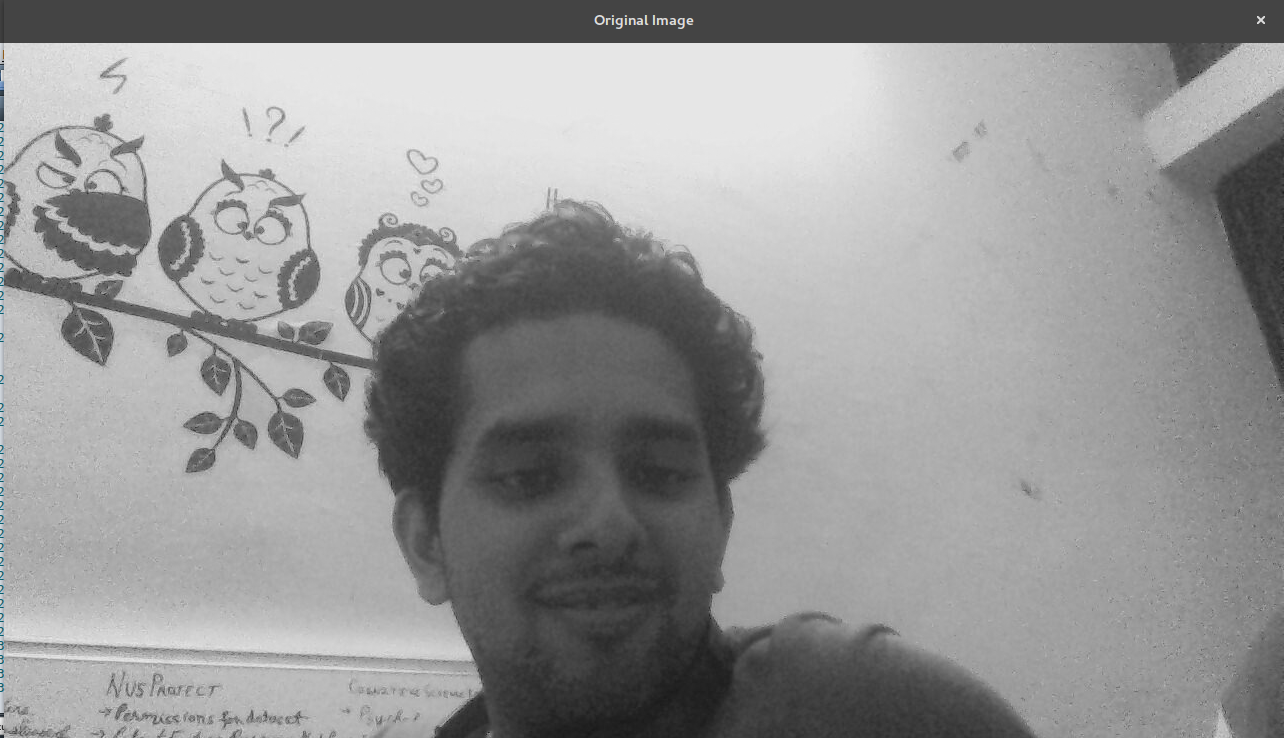
\includegraphics[scale= 0.25]{../results/divyat.png}
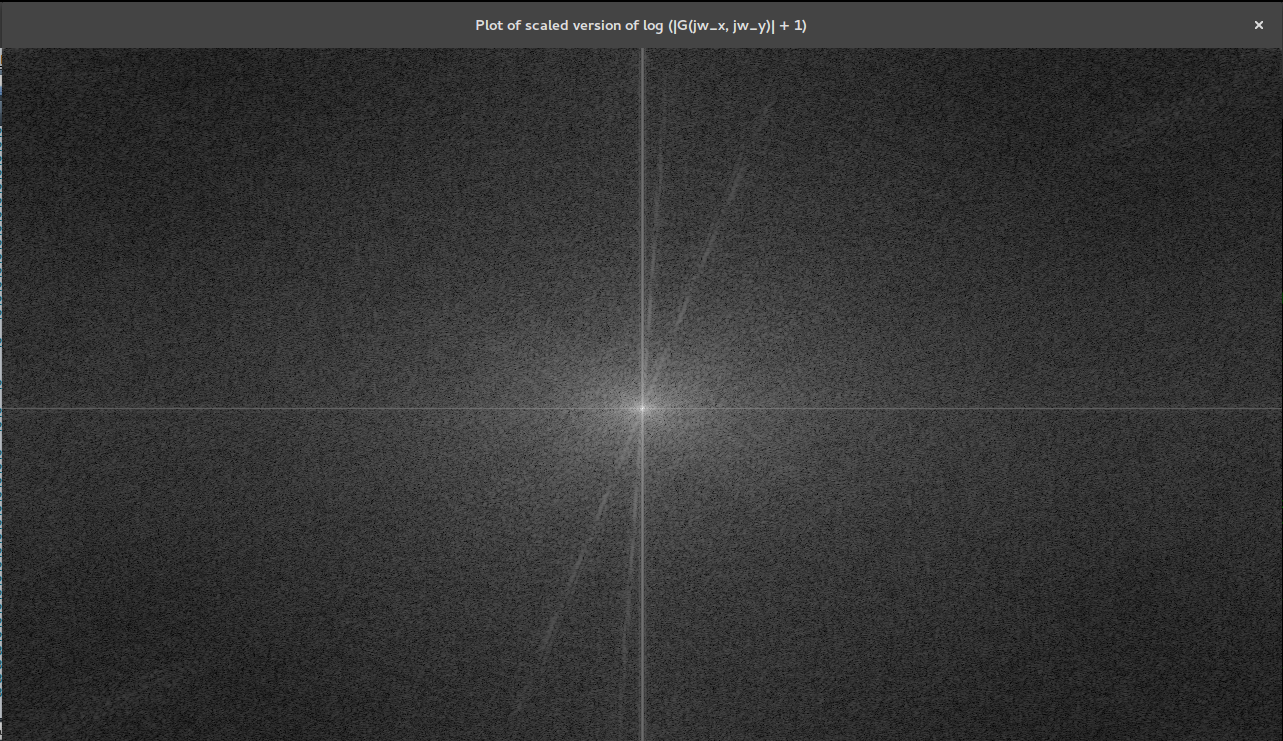
\includegraphics[scale= 0.25]{../results/divyat_spectrum.png}
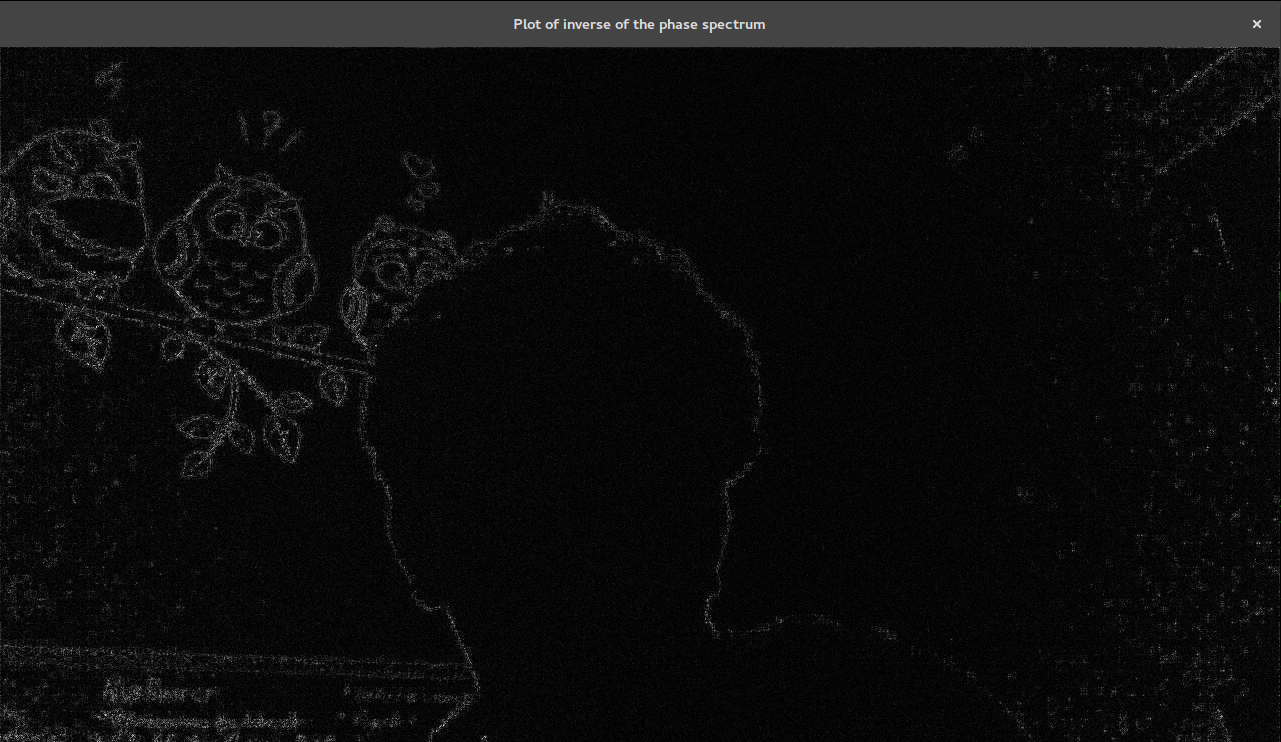
\includegraphics[scale= 0.25]{../results/divyat_phase.png}
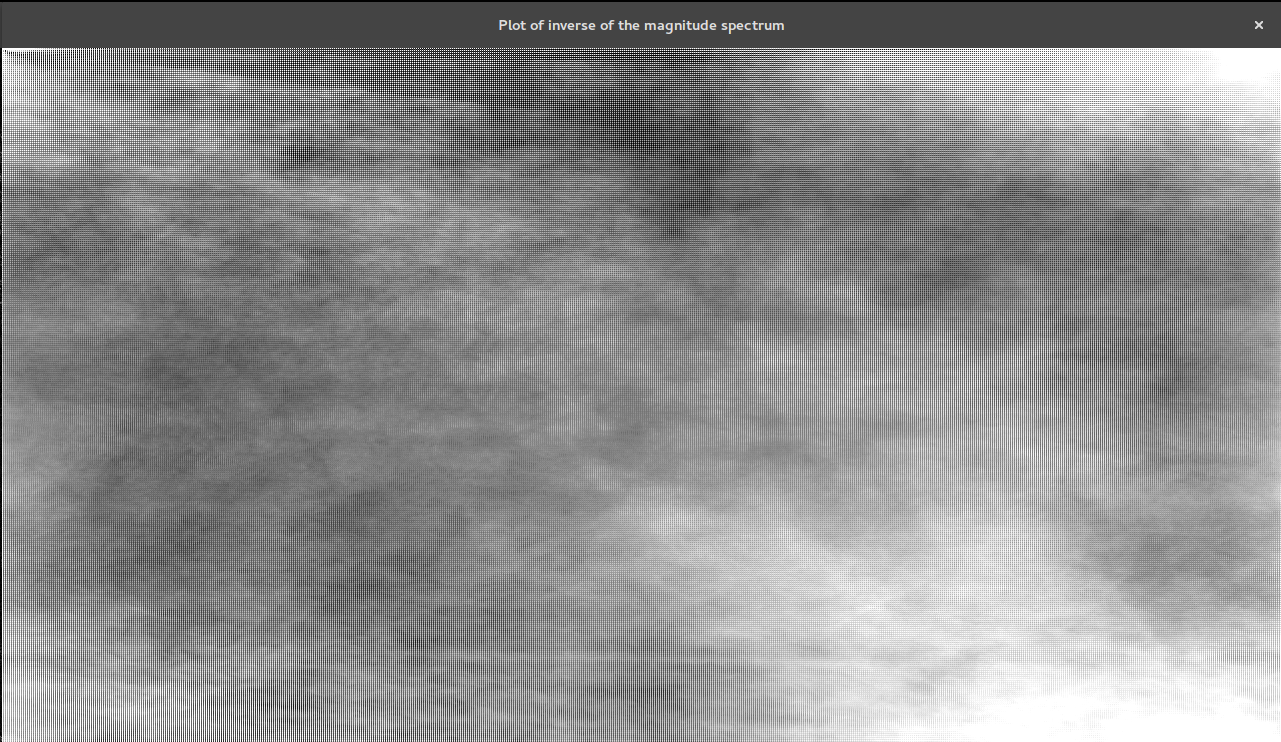
\includegraphics[scale= 0.25]{../results/divyat_magnitude.png}
\end{center}
\begin{center}
low.jpg \\
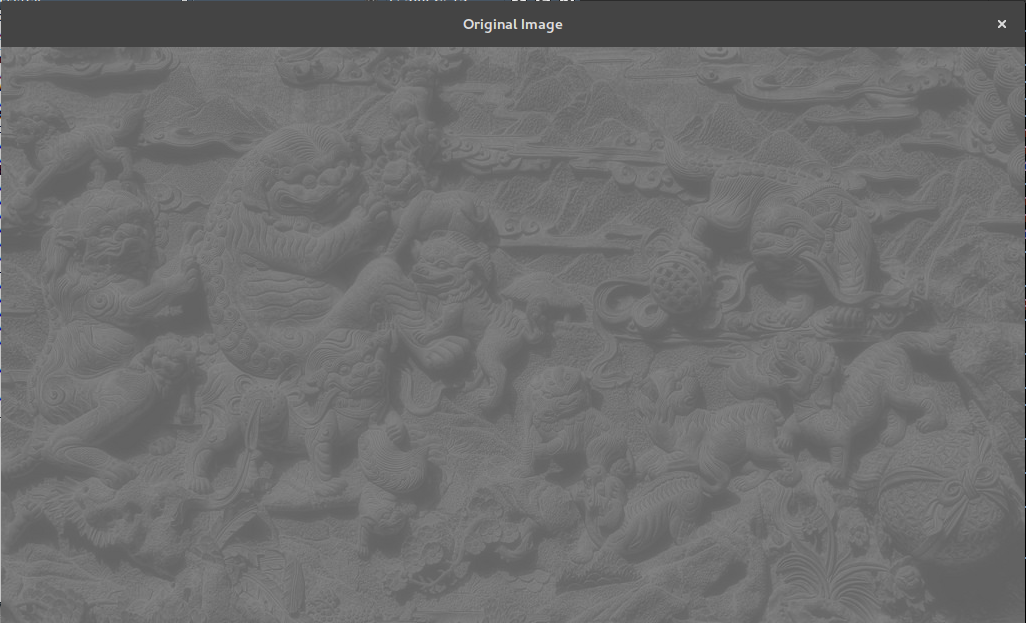
\includegraphics[scale= 0.25]{../results/low.png}
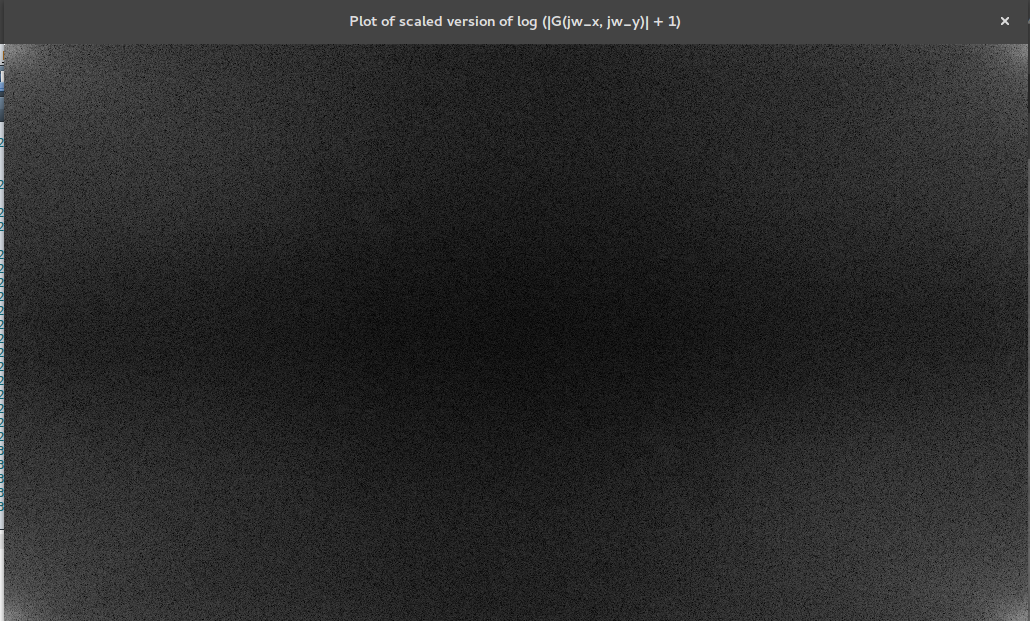
\includegraphics[scale= 0.25]{../results/low_spectrum.png}
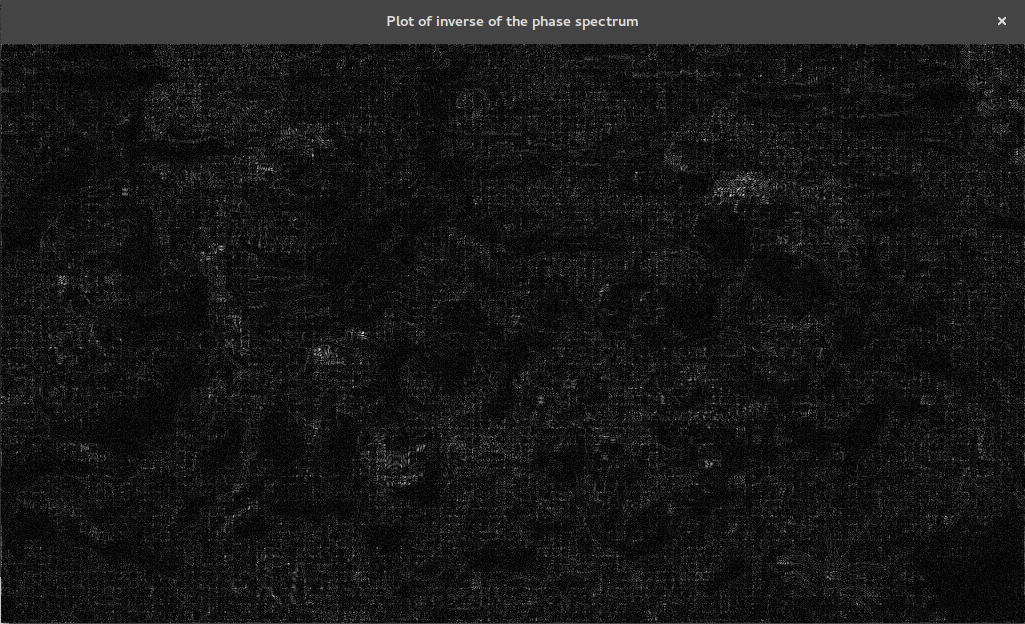
\includegraphics[scale= 0.25]{../results/low_phase.png}
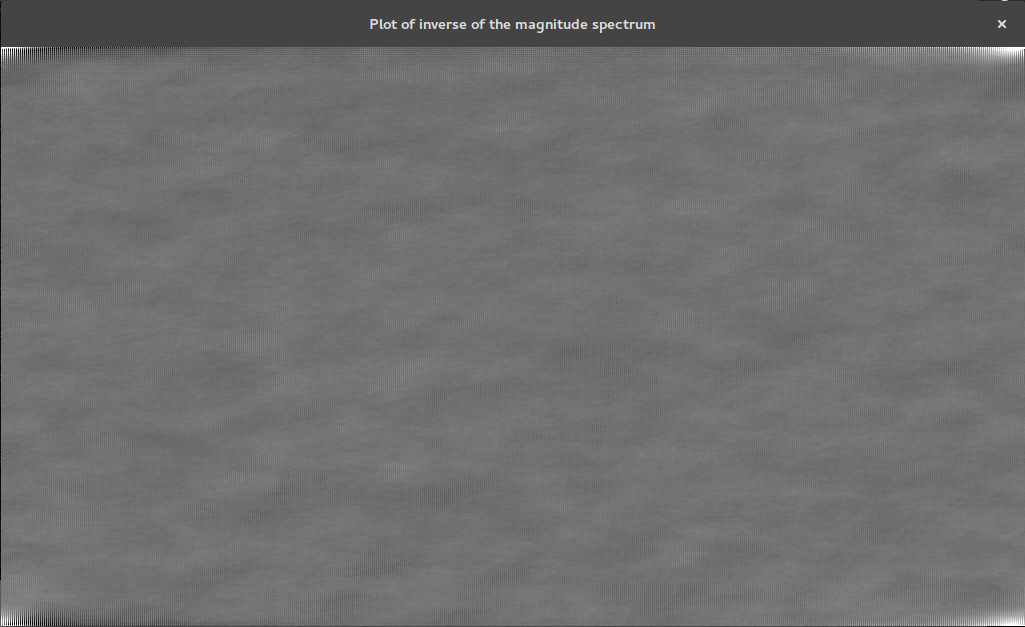
\includegraphics[scale= 0.25]{../results/low_magnitude.png}
\end{center}
\subsection*{Observations}
\subsubsection*{Reconstruction using only phase spectrum}
From the above the tests, it can be inferred that performing reconstruction using only phase information, edges are being preserved and we are losing all grey-levels of homogenous regions. From, the spectrum plots, we can infer that the lower frequency components tend to have greater values than the higher frequency ones in general images. Thus, when we remove the magnitude information, the lower frequency components are getting more suppressed than the higer frequency components, i.e. the operation is similar to a high-pass filter. This premise explains the above images obatined using only the phase spectrum.
\subsubsection*{Reconstruction using only magnitude spectrum}
The reconstruction using only magnitude spectrum appears to only contain information regarding the prominent greylevels present in the image.

\section*{Solution 7}
\begin{figure*}[h]
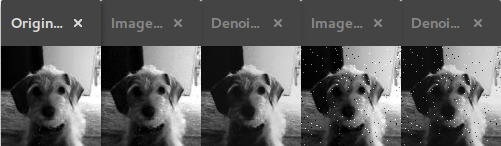
\includegraphics[scale=1.0]{../results/Q7_sigma01.png}
\caption{The images from left to right are as follows : (a) The original image (small.jpg), (b) The images with added zero-mean gaussian noise with $\sigma^2 = 0.1$, (c) The reconstucted image [b], (d) The image with impulse noise, (e) The reconstructed image [d]}
\end{figure*}

\end{document}